%\documentclass[prb]{revtex4-1}
\documentclass[11pt]{article}
%\documentclass[prb,preprint]{revtex4-1}
% Users of the {thebibliography} environment or BibTeX should use the
% scicite.sty package, downloadable from *Science* at
% www.sciencmag.org/misc/con-info.shtml .  This package should properly
% format in-text reference calls and reference-list numbers.
\usepackage{epsfig}
\usepackage{geometry}
\geometry{letterpaper}
\usepackage{graphicx}
\usepackage{amssymb}
\usepackage{epstopdf}
\usepackage{amsmath}  % needed for \tfrac, \bmatrix, etc.
\usepackage{amsfonts} % needed for bold Greek, Fraktur, and blackboard bold
\usepackage{url}
%\DeclareGraphicsRule{.tif}{png}{.png}{`convert #1 `dirname #1`/`basename #1 .tif`.png}
% Use times if you have the font installed; otherwise, comment out the
% following line.

\usepackage{times}

% The preamble here sets up a lot of new/revised commands and
% environments.  It's annoying, but please do *not* try to strip these
% out into a separate .sty file (which could lead to the loss of some
% information when we convert the file to other formats).  Instead, keep
% them in the preamble of your main LaTeX source file.


% The following parameters seem to provide a reasonable page setup.

\topmargin 0.0cm
\oddsidemargin 0.2cm
\textwidth 16cm 
\textheight 21cm
\footskip 1.0cm


%The next command sets up an environment for the abstract to your paper.

\newenvironment{sciabstract}{%
\begin{quote} \bf}
{\end{quote}}


% If your reference list includes text notes as well as references,
% include the following line; otherwise, comment it out.

%\renewcommand\refname{References and Notes}

% The following lines set up an environment for the last note in the
% reference list, which commonly includes acknowledgments of funding,
% help, etc.  It's intended for users of BibTeX or the {thebibliography}
% environment.  Users who are hand-coding their references at the end
% using a list environment such as {enumerate} can simply add another
% item at the end, and it will be numbered automatically.

\newcounter{lastnote}
\newenvironment{scilastnote}{%
\setcounter{lastnote}{\value{enumiv}}%
\addtocounter{lastnote}{+1}%
\begin{list}%
{\arabic{lastnote}.}
{\setlength{\leftmargin}{.22in}}
{\setlength{\labelsep}{.5em}}}
{\end{list}}


% Include your paper's title here

\title{Teaching Numerical Methods in the Context of Galaxy Mergers}


% Place the author information here.  Please hand-code the contact
% information and notecalls; do *not* use \footnote commands.  Let the
% author contact information appear immediately below the author names
% as shown.  We would also prefer that you don't change the type-size
% settings shown here.

\author
{\\
\\
\\
\\
A Senior Project
\\
\\
By
\\
\\
Maria Kourjanskaia
\\
\\
\\ 
\normalsize{Advisor, Dr. Jennifer Klay}
\\
\\
\normalsize{Department of Physics, California Polytechnic University SLO}\\
\\
\\
\\
\\
\\
}

% Include the date command, but leave its argument blank.

\date{\today}


                                      % Activate to display a given date or no date

\begin{document}
\baselineskip21pt
\maketitle


\newpage

\begin{center}Approval Page\end{center}
\bigskip

\begin{flushleft}
\textbf{Title: Teaching Numerical Methods in the Context of Galaxy Mergers}
\medskip

\textbf{Author: Maria Kourjanskaia}
\medskip

\textbf{Date Submitted: May 26, 2016}
\end{flushleft}

\bigskip
\bigskip
\bigskip
\bigskip
\bigskip
\bigskip
\bigskip
\bigskip
\bigskip
\bigskip
\bigskip
\bigskip
\bigskip
\bigskip
\bigskip
\bigskip
\bigskip
\bigskip
\bigskip


\begin{flushright}
Senior Project Advisor: Dr. Jennifer Klay

\bigskip
\bigskip


\line(1,0){200}

Signature
\bigskip

\line(1,0){200}

Date



\end{flushright}




\newpage

\tableofcontents

\listoftables

\listoffigures

\newpage

\section{Abstract}
Methods of teaching numerical methods to solve ordinary differential equations in the context of galaxy mergers were explored. The research published in a paper by Toomre and Toomre in 1972 describing the formation of galactic tails and bridges from close tidal interactions was adapted into a project targeting undergraduate physics students. Typically undergraduate physics students only take one Computational Physics class in which various techniques and algorithms are taught. Although it is important to study computational physics techniques, it is just as important to apply this knowledge to a problem that is representative of what computational physics researchers are investigating today. The model that was developed is capable of showing general trends in galactic evolution and is a good introduction for students who hope to expand on this topic in the future.

\section{Introduction} 

Computational physics is based upon the idea that a computer can simulate certain physical environments to produce novel scientific conclusions.  This field allows scientists to conduct experiments on the computer that are just not realistic or possible to do in the real world because of the investigation of topics involving extremely large data sets and complicated physical interactions\cite{Hjorth2008}.  This paper investigates the components and processes of modeling galaxy mergers on an undergraduate academic level.  The project outlined in this paper is derived from a paper written by Toomre and Toomre in 1972 that described the formation of galactic tails and bridges from close tidal interactions \cite{Toomre1972}. This project could be assigned to undergraduate students in an introductory computational physics class to demonstrate the capabilities and possibilities of what the field has to offer.  

The galaxy mergers project teaches students numerical methods to solve ordinary differential equations.  The galaxies modeled interact via ordinary differential equations so students are able to learn about these techniques through an applied project that is a simplified version of a cutting edge computational physics topic today \cite{Chilingarian2010}.  A lot of the time undergraduate physics students only take one computational physics class in which they learn about various techniques and algorithms that can in theory be applied to model more complicated physical situations \cite{Caballero2013}.  Although it is important to learn about the underlying theory and algorithms, it is just as important to apply this knowledge to a problem that is representative of what computational physics researchers are investigating today.  The project in this paper does in fact accomplish this goal and teaches numerical methods through application.

Although this project uses ordinary differential equations to model galaxy mergers, currently computational physics researchers use supercomputers to solve partial differential equations using the Boltzmann approximation \cite{Springel2005}.  The cutting edge research today accounts for the evolution of black holes and dark matter, star formation, and the interactions between individual stars \cite{Hung2013,Saitoh2009,Barnes1998,Bournaud2005}.  These characteristics are important in modeling galaxy mergers, but supercomputers are needed to compute all of the calculations.  Our model works well enough to see general trends in galactic shapes and is a good introduction for students who want to expand on this topic in the future.

Although Toomre and Toomre's paper dates back to 1972, it is still a good model to use for undergraduate students in a computational physics class.  Their research provided good and accurate results despite the assumptions and simplifications that they made.  Researchers today can produce more precise results and investigate a larger range of topics than in 1972, but the foundation for producing these results is still the same.  This project is an excellent introduction to the capabilities of computational physics and is a great learning opportunity for undergraduate physics students.  

\section{Background Theory}

Galaxies are a collection of stars that are orbiting around their common center of mass, interacting through gravity.  Galaxies come in various shapes and sizes, but the scientist Edwin Hubble designed a classification system for galaxies that is still used today.  He grouped galaxies into four categories including elliptical, spiral, disk, and irregular.  Today we have expanded upon these four groups, but only to add subcategories.  Today elliptical galaxies can be classified according to the ratio between their minor axis and major axis dimensions to differentiate between more circular as opposed to more elongated shapes.  Spiral galaxies are now classified with how tight or loose the spiral arms are, and whether or not there are a cluster of stars in a bar shape in the center of the galaxy.  Disk galaxies are considered to be a transition point between elliptical and spiral galaxies, and were added to the classification system by Hubble approximately 10 years after he created the original one.   Although there are galaxy classification systems in place, a galaxy does not necessarily maintain its shape throughout its life time.

Galaxies can change shape due to galactic mergers and interactions.  When one galaxy approaches or collides with another, the gravitational force between the two can be so strong that the general shapes of the galaxies can forever be changed.  For instance gravitational interactions with other galaxies have been known to morph the arms of spiral galaxies, change or add the bar structure in spiral galaxies, add features such as tidal tails, and sometimes completely merge the two galaxies together [10].  This paper examines how the positions of individual stars in one galaxy can change with an interaction of another galaxy.  This is important in the grand scheme of things, because this project allows students to predict how a galaxy's shape can morph over time in various situations.  Trends in galactic morphology are easily visible in this project despite the simplifications that were made.

Our modern understanding of cosmology indicates that a large fraction of the total matter in the universe is in fact dark matter.  Dark matter does not emit or absorb light and is therefore virtually invisible.  Dark matter is able to interact gravitationally with other matter, so it can be detected by observing trajectories of visible matter.  For example the orbital velocity of visible matter as a function of radius from the center of spiral galaxies does not follow the standard Keplerian motion one would expect for a system with most of the mass concentrated at the center.  In fact, the orbital velocities are larger which suggests that the mass increases more than expected along the galactic radius.  This phenomenon suggests the presence of dark matter in galaxies [11]. Dark matter is distributed non-uniformly throughout the universe. When modeling galaxy mergers and interactions, advanced computer models use smooth particle hydrodynamics to model the diffuse gas and dark matter components of the galaxies.  These simulations can convert the gas into new star populations while the dark matter interacts gravitationally through mean field approximations[3].  Our simplified model ignored these components of galaxies.

Supermassive black holes are believed to reside in the center of galaxies due to their strong gravitational pull in relation to their size [12].  Recently a black hole was discovered in the center of a quasar that was 12 billion times the mass of our sun [13].  It is hypothesized that super massive black holes are actually formed through galaxy mergers [14].  Since the universe is expanding, the early universe was a lot more compact and more galactic interactions were able to occur. The kind of computational modeling used in this project therefore provides students a way to study galactic mergers and the interactions of black holes in the early universe.   

\section{Model, Assumptions, and Simplifications}\label{MAS_sec}

Galaxies are very complicated entities and there are a lot of factors that can contribute to the positions and velocities of stars.  First of all, galaxies contain an uneven distribution of matter which is very difficult to model.  Second of all, the stars themselves interact gravitationally with each other despite ultimately orbiting around the galactic center.  These factors involve advanced computational techniques and equipment that is more serious than an average computer that an undergraduate student may own.  Following the example of Toomre and Toomre \cite{Toomre1972}, the simulation was simplified so that the stars in this project were treated as unit mass point objects which do not interact with each other but do interact with a large, concentrated galactic core point mass of $10^{11}$ solar masses in the center of the galaxy.  The unit-mass stars were oriented in rings around the galactic center.  The two interacting galaxies were labeled "main" and "disruptor", with unit mass stars orbiting the main galaxy but none orbiting the disruptor.  Although the disrupting galaxy could follow either hyperbolic, parabolic, or elliptical approach trajectories, this simulation only computed parabolic trajectories.  These simplifications made it possible to conduct the computations at each time step using Newtonian gravity differential equations that describe the motion. Figure \ref{geometry_fig} shows the orbital geometries and variables used in the simulation.  A description of the variables is provided in Table \ref{table1}.

\begin{figure}[h!]
%% The bracketed code determines the figure's placement:  "h" stands for 
%% "here", telling LaTeX to put the figure as close to the current location 
%% as possible.  The ! overrides LaTeX's tendency to try to find a location 
%% that it thinks is better.  But don't agonize over the exact figure placement 
%% in your submitted manuscript.  For your initial submission, just make sure 
%% each figure is reasonably close to where it's first referenced.
\centering
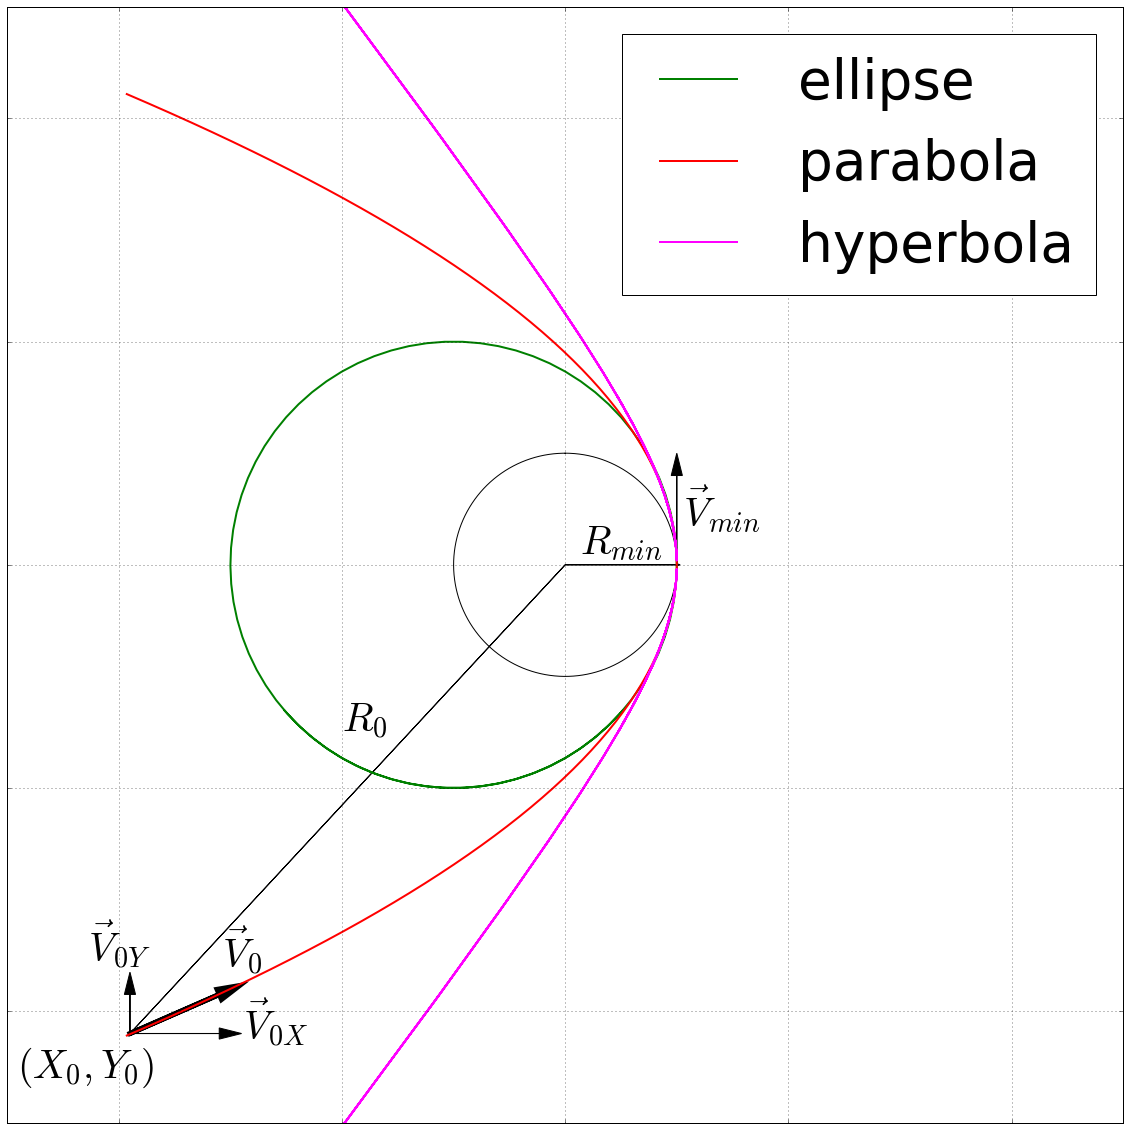
\includegraphics[width=5in]{Figure_A_1.png}
\caption{Diagram of the orbital geometry and variables.}
\label{geometry_fig}
\end{figure}

\begin{table}[h!]
\centering
\caption{Key for variables shown in Figure \ref{geometry_fig}.}
%\begin{ruledtabular}
\begin{tabular}{l p{8cm}}
% The codes above determine the horizontal alignment in each column.
% Options are l (left), r (right), c (centered), and p (paragraph).
% The p option allows an entry to be broken into multiple lines, and
% therefore requires a width specification, in this case 5 centimeters.
Variable & Description \\
\hline	% horizontal line to separate headings from data
$X_0$, $Y_0$ & Initial x and y position of disrupting galaxy \\
$\vec{V}_0$ & Initial velocity of disrupting galaxy \\
$\vec{V}_{min}$ & Minimum velocity of disrupting galaxy \\
$R_0$ & Initial separation between the two galaxies \\
$R_{min}$ & Minimum separation between the two galaxies \\
\end{tabular}
%\end{ruledtabular}
\label{table1}
\end{table}

Table \ref{table1} displays the values that a user can input into the program. Using these numbers and the constraint of a parabolic passage, the initial velocity parameters can be computed.

\begin{table}[h!]
\centering
\caption{User input values for this simulation, following the example of Toomre and Toomre.  The values are chosen such that the distance of closest approach between the two galaxies, $R_{min}$ is 25 kpc.}
%\begin{ruledtabular}
\begin{tabular}{l l l l l}
% The codes above determine the horizontal alignment in each column.
% Options are l (left), r (right), c (centered), and p (paragraph).
% The p option allows an entry to be broken into multiple lines, and
% therefore requires a width specification, in this case 5 centimeters.
Merger Case & $Rx_0$(Mpc) & $Ry_0$(Mpc) & $M$($M_{sol}$) & $S$($M_{sol}$) \\
\hline	% horizontal line to separate headings from data
Direct Passage & -39 & -80 & $10^{11}$ & $10^{11}$ \\
Retrograde Passage & -39 & 80 & $10^{11}$ & $10^{11}$ \\
Light Mass Disruptor & -39 & -80 & $10^{11}$ & 0.25$\times10^{11}$ \\
Heavy Mass Disruptor & -39 & -80 & $10^{11}$ & 4$\times10^{11}$ \\
\end{tabular}
%\end{ruledtabular}
\label{table2}
\end{table}


This project consisted of two galaxies.  One galaxy contained stars and remained at the origin of our reference frame, whereas the other galaxy had a perfectly parabolic trajectory (in relation to the origin) and was simply a point mass with no stars.  This configuration allows one to clearly observe the evolution of star positions in a galaxy merger.  Additionally the only cases that were examined in this project were direct passage, retrograde passage, light mass disruptor and heavy mass disruptor cases which will soon be explained. 

After $R_{min}$ was set, it was possible to calculate the initial velocity parameters of the disrupting galaxy.  The disrupting galaxy was set to follow a perfect parabolic trajectory, so the initial velocity conditions were extremely important. These conditions pave the trajectory that the galaxy will follow.  First, the Vis-Viva equation was used to determine the minimum velocity of the disrupting galaxy that occurred at $R_{min}$.  

\begin{equation}
v^2 = GM(\frac{2}{r} - \frac{1}{a}) 
\end{equation}

where $v$ is the relative speed between two bodies, $r$ is the separation between two bodies, $M$ is the mass of the central body, $G$ is the gravitational constant, and $a$ is the semi major axis.

With parabolas the semi-major axis approaches infinity, so the Vis-Viva equation can be reduced to

\begin{equation}
v_{min}= \sqrt{\frac{2GM}{R_{min}^2}}
\end{equation}

Using $v_{min}$, the angular momentum, $\ell_{min}$ can be calculated from

\begin{equation}
\ell = \ell_{min} = r_{min}v_{min}= constant 
\end{equation}

which is constant for the entire trajectory of the disrupting galaxy.  This angular momentum value can be used to determine the parameters of the general equation of a parabola described by

\begin{equation}
y^2 = c^2 - 2cx
\end{equation}

where the parameter $c$ is related to the masses and angular momentum through

\begin{equation}
c = \frac{\ell^2}{GM_1M_2\mu}
\label{c_eqn}
\end{equation}

\begin{equation}
\mu = \frac{M_1M_2}{M_1 + M_2}
\label{mu_eqn}
\end{equation}

A starting value for the initial y position, $Y_0$, was set, and the general equation of the parabola was used to determine the corresponding $X_0$ value.  These coordinates were ultimately used to determine the initial separation value between the two galaxies $R_0$ which can be calculated  

\begin{equation}
R_0 = \sqrt{(X_0^2) + (Y_0^2)}
\label{R0_eqn}
\end{equation}

From $R_0$, the magnitude of the initial velocity can be determined from 

\begin{equation}
V_0= \sqrt{\frac{2GM}{R_0^2}}
\label{V0_eqn}
\end{equation}

which is tangent to the parabolic trajectory at that location.  The x and y components of the velocity vector are then calculated.

To compute the magnitudes of the initial velocities of the stars orbiting the main galaxy in concentric rings, the modified Vis-Viva equation for the case of circular orbits 

\begin{equation}
v_0= \sqrt{\frac{2GM}{r_0^2}}
\end{equation}

can be used.  Then as before, the vector components are determined from the tangent of the circle at each initial position.

With the initial conditions set, the calculation of the subsequent position and velocities for each time step under Newtonian gravitational forces can be undertaken.  The positions of the unit-mass stars are described by the differential equation

\begin{equation}
\ddot{\mathbf{r}} = -\gamma \left\{ \frac{M}{r^3}\mathbf{r} -\frac{S}{\rho^3}\boldsymbol{\rho} + \frac{S}{R^3}\boldsymbol\Re \right\}
\label{star_eqn}
\end{equation}

and that of the disrupting galaxy by

\begin{equation}
\ddot{\boldsymbol\Re} = -\gamma \frac{M+S}{R^3}\boldsymbol\Re
\label{disruptor_eqn}
\end{equation}

with the variables and constants defined as follows:

\begin{itemize}
\item $\gamma$ is the Gravitational constant.
\item $M$ is the central mass of the main galaxy and $S$ is the central mass of the disrupting galaxy
\item $\mathbf{r}$ is the radius vector from mass $M$ to massless point particle $m$, representing a single (unit-mass) star in the outer disk of the main galaxy.
\item $\boldsymbol\Re$ is the radius vector from $M$ to $S$.
\item $\boldsymbol{\rho} = \boldsymbol{\Re} - \boldsymbol{r}$
\end{itemize}

Figure \ref{coords_fig} shows the coordinate system for the galaxy interactions.

\begin{figure}[h!]
%% The bracketed code determines the figure's placement:  "h" stands for 
%% "here", telling LaTeX to put the figure as close to the current location 
%% as possible.  The ! overrides LaTeX's tendency to try to find a location 
%% that it thinks is better.  But don't agonize over the exact figure placement 
%% in your submitted manuscript.  For your initial submission, just make sure 
%% each figure is reasonably close to where it's first referenced.
\centering
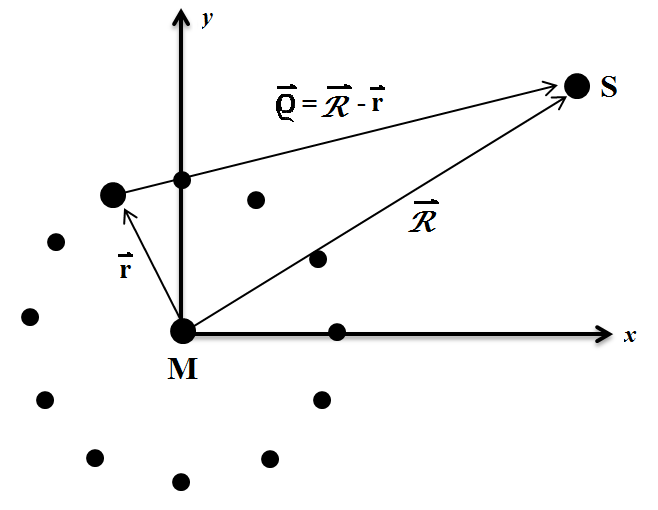
\includegraphics[width=5in]{Figure2.png}
\caption{Coordinate system for galaxy interaction.}
\label{coords_fig}
\end{figure}

\section{Set Up of the General Code}\label{Setup_sec}

To begin with, the stationary galaxy containing stars is set at the origin.  The bulk of this galaxy is represented as a point mass, which means that all of its mass is concentrated at a point in its center.  The galaxy contains 120 unit-mass stars which are initially distributed throughout 5 discrete, concentric rings around the galaxy.  Each ring contains 12, 18, 24, 30, and 36 stars respectively (the inner most ring contains 12 stars).  For the direct passage, retrograde passage, and light mass disruptor cases the concentric rings are placed at exactly 20, 30, 40, 50, and 60 percent of the minimum distance between the two galaxies $R_{min}$, as shown in Figure \ref{starlocdirect_fig}. 

\begin{figure}[h!]
%% The bracketed code determines the figure's placement:  "h" stands for 
%% "here", telling LaTeX to put the figure as close to the current location 
%% as possible.  The ! overrides LaTeX's tendency to try to find a location 
%% that it thinks is better.  But don't agonize over the exact figure placement 
%% in your submitted manuscript.  For your initial submission, just make sure 
%% each figure is reasonably close to where it's first referenced.
\centering
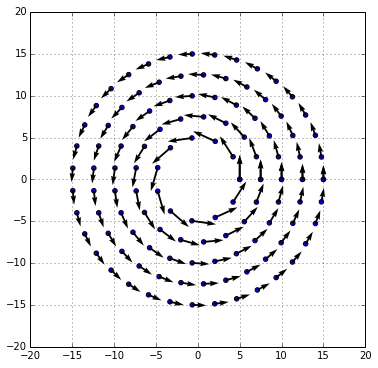
\includegraphics[width=5in]{DirectPassageImage.png}
\caption{Locations of stars in stationary galaxy for direct, retrograde and light mass disruptor cases.}
\label{starlocdirect_fig}
\end{figure}

On the other hand, in the heavy mass disruptor case the rings are more tightly placed at 12, 18, 24, 30, and 36 percent of $R_{min}$, as in Figure \ref{starlocheavy_fig}.

\begin{figure}[h!]
%% The bracketed code determines the figure's placement:  "h" stands for 
%% "here", telling LaTeX to put the figure as close to the current location 
%% as possible.  The ! overrides LaTeX's tendency to try to find a location 
%% that it thinks is better.  But don't agonize over the exact figure placement 
%% in your submitted manuscript.  For your initial submission, just make sure 
%% each figure is reasonably close to where it's first referenced.
\centering
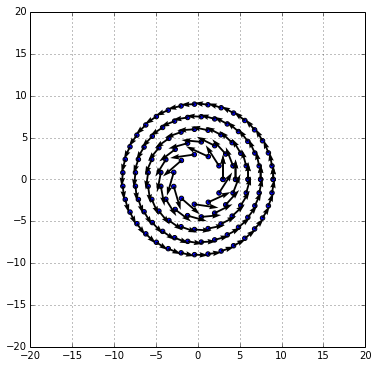
\includegraphics[width=5in]{HeavyPassageImage.png}
\caption{Stationary galaxy for heavy mass disruptor case.}
\label{starlocheavy_fig}
\end{figure}

In all cases this minimum distance ($R_{min}$) is set at 25 kpc.  The initial time was set to $t$ = 0 and the time step was set to exactly $10^8$ years.  In all of the featured cases, the heavier mass was set to $10^{11}$ solar masses.  To compute and visualize the simulations, several Python-based numerical tools in the NumPy, Matplotlib, and SciPy packages were used, including SciPy's \texttt{odeint} differential equation integrator and the iPython interact features.  Each of the main program functions are described next.\\

\textbf{\texttt{Set\_Init\_R\_Cond(Ry0, M, S):}}

This function was written to set the initial conditions of the disturbing galaxy, taking as inputs the initial vertical position of the disturbing galaxy (\texttt{Ry0} = $Y_0$), the mass of the stationary galaxy (\texttt{M}), and the mass of the disturbing galaxy (\texttt{S}).  The minimum separation distance between the two galaxies, $R_{min}$, is set at 25 kpc.  The minimum velocity at $R_{min}$ is determined using equation \ref{V0_eqn} allowing for variable values of the galactic masses.  The angular momentum and $c$ parameter of the parabolic trajectory are determined using these values according to equations \ref{c_eqn} and \ref{mu_eqn}.  The $c$ parameter is used to compute the corresponding initial horizontal position of the disturbing galaxy ($X_0$) which in turn can be used to compute the distance of the disturbing galaxy from the origin ($R_0$) according to equation \ref{R0_eqn}.  The unit tangent vectors are then determined for the parabolic trajectory and are used to set the initial X and Y velocities of the disturbing galaxy.  The function returns initial X and Y positions and velocities of the disturbing galaxy.\\

\textbf{\texttt{Ring(particles, percent, G, M):}}

This function was set up to produce initial conditions of the stars around the stationary galaxy.  This function takes in arguments called \texttt{particles}, \texttt{percent}, \texttt{G}, and \texttt{M}.  The variable \texttt{particles} describes the number of stars that are desired in one ring around the center of the stationary galaxy.  The variable \texttt{percent} describes at what percentage of $R_{min}$ the distance between each star and the origin of the stationary galaxy should be. Lastly, \texttt{G} is used for the Universal gravitational constant in appropriate units, and \texttt{M} is the desired mass of the stationary galaxy. First the radius of each star is defined as a percent of the $R_{min}$ value set in the previous function.  The stars can be plotted along a circular trajectory around the origin of the stationary galaxy.  The arc length of each trajectory is divided among each ring of stars so that the stars are spaced equally apart.   This is accomplished through a while loop that fills the star locations in an initially empty array with each turn of the loop.  The loop runs as many times as there are stars to be created.   Although the star locations are initially computed in polar coordinates, their positions are converted to Cartesian coordinates and appended to an empty list.  The initial velocity conditions are also created using equation \ref{V0_eqn}.  These velocities are tangent to the circle that the stars are plotted along.  This function returns an array of star positions and an array of star velocities. \\

\textbf{\texttt{Init\_rings (G,M):}}

This function takes as inputs the gravitational constant in appropriate units (\texttt{G}) and the stationary galactic mass (\texttt{M}).  The previous `Ring` function sets up all of the formulas using variables to set the initial positions and velocities of the stars in a single ring.  This function uses the \texttt{Ring} function to build the full list of star positions and velocities for the galaxy.  There are two ring initialization functions to allow for different numbers of stars and different percentage locations used for the different cases.  Specifically, each ring in every case contains 12, 18, 24, 30, and 36 stars respectively (the inner most ring contains 12 stars).  For the direct passage, retrograde passage, and light mass disruptor cases the concentric rings are placed at exactly 20, 30, 40, 50, and 60 percent of the minimum distance between the two galaxies ($R_{min}$) while in the heavy mass disruptor case the rings are placed at 12, 18, 24, 30, and 36 percent of $R_{min}$.  This function returns an array of star position values and an array of star velocity values.\\

\textbf{\texttt{Unpack\_rings\_vel(rings, velocity):}}

This function takes in the arguments \texttt{rings} and \texttt{velocity} which are the outputs from \texttt{Init\_rings}.  The purpose of this function is to organize the information in the rings and velocity arrays into separate lists of x positions of stars, y positions of stars, x velocities of stars, and y velocities of stars.  This can be accomplished by writing a for loop that loops through the rings and velocity arrays and selects the desired information using indexing techniques and appending the proper information to an initially empty list.  This function returns four separate arrays that describe the x and y positions and velocities of the stars.\\

\textbf{\texttt{Derivgalaxy(y, t, M, S):}}

This function takes as inputs an array containing all of the position and velocity information of the disturbing and stationary galaxies (\texttt{y}), the period of time to be examined (\texttt{t}), and the stationary (\texttt{S}) and disrupting (\texttt{M}) galactic masses.  The disrupting galaxy and star locations and velocities for each time step are computed using equations \ref{star_eqn} and \ref{disruptor_eqn} with SciPy's \texttt{odeint} differential equation integrator to describe the position of each star and disrupting galaxy over time.  This function outputs an array of the x and y velocity and acceleration values of each star and disrupting galaxy.\\

\textbf{\texttt{Make\_Master\_Array(Case = 1, Rx0 = -39, Ry0 = -80, M = 1.0e11, S = 1.0e11):}}

This function is the main calling function to compute the full simulation.  The inputs are which case to simulate, (\texttt{Case}=1-4), the starting x,y position of the disrupting galaxy (\texttt{Rx0}, \texttt{Ry0}), and the masses of the stationary (\texttt{M}) and disrupting galaxy (\texttt{S}).  This function sequentially calls all of the previous functions according the case number that is to be examined.  This could be achieved by using \texttt{if} and \texttt{elif} statements to run certain functions if a certain case is called.   As the \texttt{Derivgalaxy} function loops over each time step the results are appended at each time step to a master array.  The purpose of this is to run the calculation one time in its entirety and to store the results in an array for plotting and quick referencing.  This function outputs a complete master array containing all of the information of the stars and disrupting galaxy at each time step.\\

\textbf{\texttt{Make\_Plot\_stars(results, M, S, t, dt):}}

This function generates the visualization of the galaxy interaction.  It takes as inputs the results of the \texttt{Make\_Master\_Array} function (\texttt{results}), the masses of the stationary (\texttt{M}) and disrupting (\texttt{S}) galaxies, the total time the user would like to examine (\texttt{t}), and the time steps (\texttt{dt}) which were integrated over.  This function sets the stationary galaxy location at the origin and ensures that all of the stars will orbit and move in reference to the set origin at the stationary galactic center.  The trajectories are plotted using an iPython \texttt{interact} widget tool that allows the user to slide through all of the calculated time steps and observe the evolution of the galaxies in a movie-like layout. \\

\textbf{\texttt{Make\_Plots\_Yellow\_Star(results, M, S, t, dt, Yellowstar):}}

This function is almost identical to the previous \texttt{Make\_Plot\_Stars} function, except it contains an extra argument called \texttt{Yellowstar} that allows the user to index a certain star in the master array to be colored yellow (all of the other stars are red).  All stars are plotted as before but a second loop runs to draw second yellow star on top of the existing red one.  Although two stars are plotted in one location, the user only sees the yellow star that is covering the red one. 

\section{Challenges}

When creating the galaxy mergers model, one must be aware of some challenges that can impede one's progress.  First of all, it is important to set initial position and velocity conditions according to the equations listed above in Section \ref{MAS_sec}.  If arbitrary values are set instead, the disrupting galaxy will not follow a perfect parabolic approach and the stars will not move along realistic trajectories.

Another challenge to be aware of is setting the proper time step.  If one sets a time step that is too large, the positions of the stars are not calculated frequently enough and they may jump to the origin when the disrupting galaxy is close.  This problem occurs because of a numerical precision problem that results in the magnification of error.  The best time step to be used for this project was found through experimentation to be 0.007.

\section{Validation}

To validate the correctness of our simulation, we compared our results to the four cases studied by Toomre and Toomre \cite{Toomre1972}.  The four cases were direct passage, retrograde passage, light mass disruptor and heavy mass disruptor.  Direct passage occurs when the stationary galaxy and disrupting galaxy have equal mass, and the disrupting galaxy approaches the stationary one along a parabola with the same direction that the stars are orbiting.   Retrograde passage is very similar except the disrupting galaxy approaches in the opposite direction that the stars are orbiting.  A way to visualize these concepts is that the stars are orbiting counter clockwise and in a direct passage the galaxy approaches counter clockwise as well, whereas in the retrograde passage the disruptor follows a clockwise trajectory.  A light mass disruptor was also modeled where the disrupting galaxy approached along a direct approach, but had only a quarter of the mass of the stationary galaxy.  The heavy mass disruptor on the other hand was also a direct approach, but the disruptor had four times the galactic mass of the stationary galaxy.  We confirmed that our simulations of these cases matched the results published in \cite{Toomre1972}, demonstrating that it can be used to explore new configurations with confidence that the physics is valid. 

\section{Applications and Future Extensions}

After a student gets this project working, they may build upon the existing program with the following suggestions.  First, it may be interesting to examine the trajectory of a single star and follow its path.  One way to do this is to color a particular star in a different color to make it stand out amongst the other stars.  The method to accomplish this is described in Section \ref{Setup_sec} under the \texttt{Make\_yellow\_star} description. This modification allows students to see which stars are transferred to the disturbing galaxy and which stars stay with their own galaxy.  

Another modification may be to add stars to the disturbing galaxy following similar rules as modeling stars around the stationary galaxy.  It would be interesting for a student to examine how the different stars mix together over time by color coding the stars based on which galaxy they came from.  Also the student can manipulate the tilts of the interacting galaxies and study how the star trajectories are affected with this modification.  

Finally it would be interesting to include gravitational interactions between the stars.  This suggestion would take the most computing power and therefore it is recommended for a student to start with only three stars.  Once a student accomplishes this extension with three stars, they may add more as long as their computer can process the information. 

\section{Conclusion}

Computational Physics is a very broad field that covers many interesting topics.  This project focuses on modeling galaxy interactions, a sub-topic of astrophysics and cosmology.  Galaxies have many complicated factors such as dark matter, black holes, and star-star interactions that computational physicists must model on super computers. Super computers are not commonly available to undergraduate physics students, therefore this project was created to let students model galaxies using the iPython notebook on their laptops.  The project was modeled after the 1972 Toomre and Toomre paper that described the formation of galactic tails and bridges.  Toomre and Toomre imposed certain simplifications on their model including unit-mass stars, no dark matter or black holes, and a finite number of particles to track.  These assumptions were then adopted into this project.  Although the model is not as precise as  cutting-edge research that is currently being conducted on galaxy mergers, the model is definitely good enough to see general trends and is therefore interesting for undergraduates to study.   

\section*{Acknowledgments}

I would like to thank the College Based Academic Fee (CBF) for funding my research.  This money allowed me to spend my summer developing this project into what it has become.  Additionally I would like to acknowledge the Spring 2014 Physics on a Computer class that introduced me to the topic of modeling Galaxy Mergers.  This class is really where this project began!  Last of all I would like to thank my wonderful advisor Jennifer Klay for her patience and hard work in making this project a reality.  

%\end{acknowledgments}


\begin{thebibliography}{99}
% The numeral (here 99) in curly braces is nominally the number of entries in
% the bibliography. It's supposed to affect the amount of space around the
% numerical labels, so only the number of digits should matter--and even that
% seems to make no discernible difference.

\bibitem{Hjorth2008} M. Hjorth-Jensen, ``Computational Physics'', University of Oslo (2008) \url{http://www.cec.uchile.cl/cinetica/pcordero/MC_libros/Hjorth-Jensen2008.pdf}

\bibitem{Toomre1972} A. Toomre, J. Toomre, ``Galactic Bridges and Tails'', The Astrophysical Journal 178, 623-666 (1972) \url{http://articles.adsabs.harvard.edu/cgi-bin/nph-iarticle_query?1972ApJ...178..623T&data_type=PDF_HIGH&whole_paper=YES&type=PRINTER&filetype=.pdf}

\bibitem{Chilingarian2010}I. V. Chilingarian, P. Di Matteo, F. Combes, A.-L. Melchior, and B. Semelin, ``The GalMer database: galaxy mergers in the virtual observatory'', Astronomy \& Astrophysics 518, A61 (2010) \url{http://www.aanda.org/articles/aa/pdf/2010/10/aa12938-09.pdf}

\bibitem{Caballero2013} M. Caballero, S. Pollock, ``A Model for Incorporating Computation Without Changing the Course: An example from middle-division classical mechanics'', Am. J. Phys. 82, 231 (2014) \url{http://scitation.aip.org/content/aapt/journal/ajp/82/3/10.1119/1.4837437}

\bibitem{Springel2005} V. Springel, ``The cosmological simulation code GADGET-2'', Mon. Not. R. Astron. Soc. 364, 1105-1134 (2005) \url{http://www.mpa-garching.mpg.de/gadget/gadget2-paper.pdf}	 
\bibitem{Hung2013} C. L. Hung, D. B. Sanders, C. M. Casey, N. Lee, J. E. Barnes, P. Capak, J. S. Kartaltepe, M. Koss, K. L. Larson, E. Le Floc'h, K. Lockhart, A. W. S. Man, A. W. Mann, L. Riguccini, N. Scoville, M. Symeonidis, ``The Role of Galaxy Interaction in the SFR-M * Relation: Characterizing Morphological Properties of Herschel-selected Galaxies at 0.2 $<$ z $<$ 1.5'', The Astrophysical Journal, Volume 778, Issue 2, article id. 129, 13 pp. (2013) \url{http://adsabs.harvard.edu/abs/2013ApJ...778..129H}

\bibitem{Saitoh2009} T. Saitoh, H. Daisaka, E. Kokubo, J. Makino, T. Okamoto, K. Tomisaka, K. Wada, N. Yoshida, ``Toward First-Principle Simulations of Galaxy Formation: II. Shock-Induced Starburst at a Collision Interface during the First Encounter of Interacting Galaxies'', Publ Astron Soc Jpn 61 (3): 481-486 (2009) \url{http://pasj.oxfordjournals.org/content/61/3/481.short}

\bibitem{Barnes1998} J.  Barnes, ``Galaxy Interactions'', arXiv:astro-ph/9811092 (1998) \url{http://ned.ipac.caltech.edu/level5/Barnes2/paper.pdf}

\bibitem{Bournaud2005} F. Bournaud, C. J. Jog, F. Combes, ``Galaxy mergers with various mass ratios: Properties of remnants'', Astronomy \& Astrophysics 437, 69-85 (2005) \url{http://www.aanda.org/articles/aa/pdf/2005/25/aa2036-04.pdf}

\bibitem{Buta2006} R. Buta, ``Galaxies: Classification'', Encyclopedia of Astronomy and Astrophysics, Institute of Physics Publishing (2006) \url{http://www.astro.caltech.edu/~george/ay21/eaa/eaa-classif.pdf}
	
\bibitem{Freeman} K. Freeman, ``Dark Matter in Galaxies'', Encyclopedia of Astronomy and Astrophysics, Institute of Physics Publishing (2006) \url{http://www.astro.caltech.edu/~george/ay20/eaa-darkmatter-obs.pdf}

\bibitem{Madejski2003} G. Madejski, ``Black Holes in Active Galactic Nuclei'', SLAC-PUB-9702 (2003) \url{http://www3.mpifr-bonn.mpg.de/staff/mmassi/slac-pub-9702.pdf}

\bibitem{Wu2015} X. B. Wu, F. Wang, X. Fan, W. Yi,	W. Zuo, F. Bian, L. Jiang, I. McGreer, R. Wang,	J. Yang, Q. Yang, D. Thompson, Y. Beletsky, ``An ultraluminous quasar with a twelve-billion-solar-mass black hole at redshift 6.30'', Nature 518, 512-515 (2015) \url{http://www.nature.com/articles/nature14241.epdf}

\bibitem{Mayer2007} Lucio Mayer, Stelios Kazantzidis, Piero Madau, Monica Colpi, Thomas Quinn, James Wadsley, ``Rapid formation of supermassive black hole binaries
in galaxy mergers with gas``, Science 316, 1874-1877 (2007) \url{http://www.slac.stanford.edu/cgi-wrap/getdoc/slac-pub-13168.pdf}

\end{thebibliography}
%\appendix

%\section{Research Groups and Opportunities}

%\begin{table}[htdp]%\begin{center}\begin{tabular}{ccccc}\hline Organization & Group Leader & Contact Info & Webpage & Focus \\\hline Cornell University & George G. Malliaras & ggm1@cornell.edu & people.ccmr.cornell.edu/~george/ & Small Molecule/PDMS \\\hline R.U.G. &  &   &   &   \\\hline University of Washington &  &   &   &   \\\hline Berkeley &  &   &   &   \\\hline California Polytechnic State University &  &   &   &   \\\hline UC Santa Barbara &  &   &   &   \\\hline UC Santa Cruz &  &   &   &   \\\hline Stanford &  &   &   &   \\\hline Princeton &   &   &   &  \end{tabular} \caption{Research Groups}%\end{center}%\label{defaulttable}%\end{table}


%\section{CSUS 19th Annual Student Research Competition Entry}

\end{document}


